\documentclass{beamer}
\usepackage[T1]{fontenc}
\usepackage[utf8]{inputenc}
\usepackage[english]{babel}
\usepackage{graphicx}
\usepackage{subfig}
\usepackage{colortbl}
\usepackage{tikz}
\usepackage{bm}
\usepackage{listings}

%listins
\lstset{
  language=C++,
  frame=single,
  keywordstyle=\color{magenta}\bfseries,
  basicstyle=\footnotesize,
  commentstyle=\color{green}\itshape,
  stringstyle=\color{blue},
  showstringspaces=true,
  showspaces=false,
  breaklines=true,
  breakatwhitespace=true,
  tabsize=2}


\graphicspath{{Images/}}

\usetheme{Hannover}

\beamertemplatenavigationsymbolsempty
\def\swidth{1.6cm}
\setbeamersize{sidebar width left=\swidth}
\setbeamertemplate{sidebar left}{
  {\usebeamerfont{title in sidebar}%
    \vskip1.5em%
    \usebeamercolor[fg]{title in sidebar}%
    \insertshorttitle[width=\swidth,center,respectlinebreaks]\par%
    \vskip1.25em%
  }%
  {%
    \usebeamercolor[fg]{author in sidebar}%
    \usebeamerfont{author in sidebar}%
    \insertshortauthor[width=\swidth,center,respectlinebreaks]\par%
    \vskip1.25em%
  }%
  \hbox to2cm{\hss\insertlogo\hss}
  \vskip1.25em%
  \insertverticalnavigation{\swidth}%
  \vfill
  \hbox to2cm{\hskip0.6cm\usebeamerfont{subsection in
      sidebar}\strut\usebeamercolor[fg]{subsection in
      sidebar}\insertframenumber/\inserttotalframenumber\hfill}%
  \vskip3pt%
}%

\definecolor{bleufonce}{rgb}{0.1,0.1,0.8}
\definecolor{grisbleu}{rgb}{0.8,0.8,0.9}
\definecolor{rougefonce}{rgb}{0.8,0.1,0.1}
\definecolor{grisrouge}{rgb}{0.9,0.8,0.8}
\definecolor{vertfonce}{rgb}{0.1,0.8,0.1}
\definecolor{grisvert}{rgb}{0.8,0.9,0.8}
\definecolor{bleuunistra}{RGB}{15,80,150}
\setbeamercolor{palette quaternary}{fg=white,bg=bleuunistra}
\setbeamercolor{titlelike}{parent=palette quaternary}

\setbeamertemplate{blocks}[rounded][shadow=true] 
\setbeamercolor{block title}{bg=bleufonce,fg=white}
\setbeamercolor{block body}{bg=grisbleu}
\setbeamercolor{block title alerted}{bg=rougefonce,fg=white}
\setbeamercolor{block body alerted}{bg=grisrouge}
\setbeamercolor{block title example}{bg=vertfonce,fg=white}
\setbeamercolor{block body example}{bg=grisvert}

\newtheorem{pb}{Problem}
\newcommand{\R}{{\mathbb{R}}}
\newcommand{\Z}{{\bm{\mathcal{Z}}}}
\newcommand{\PP}{{\mathbb{P}}}
\newcommand{\TT}{{\bm{\mathcal{T}}}}
\newcommand{\NN}{{\bm{\mathcal{N}}}}
\newcommand{\LLL}{{\bm{\mathcal{L}}}}
\newcommand{\grad}{{\nabla}}
\newcommand{\laplace}{{\Delta}}
\newcommand{\curl}{{\nabla\times}}
\newcommand{\curll}{{\nabla^2\times}}
\renewcommand{\div}{{\nabla\cdot}}
\newcommand{\restr}{{\big\rvert_{\partial\Omega}}}
\newcommand{\taille}{0.4}
\newcommand{\taillem}{0.5}
\newcommand{\tailleg}{0.7}
\newcommand{\Ctaille}{0.5}
\newcommand{\Ctaillem}{0.6}
\newcommand{\Ctailleg}{0.8}

\title[$NS^2_{++}$]{PEPS Project $NS^2_{++}$}
\subtitle{A non standard strategy for solving the incompressible Navier-Stokes equations in Feel++}
\author[Romain Hild]{Romain Hild \inst{1} \and Christophe Prud'homme \inst{1}\\ \and Philippe Gilotte \inst{2} \and Benjamin Surowiec \inst{2}}
\institute[shortinst]{\inst{1} Université de Strasbourg \and \inst{2} Plastic Omnium Auto Exterior Services}

\begin{document}

\begin{frame}
  \makebox[\textwidth][c]{
\includegraphics[scale=0.14]{uds.jpg}
\includegraphics[scale=0.09]{po.jpg}}
  \titlepage
\end{frame}

\begin{frame}{Plastic Omnium}
  \begin{columns}[onlytextwidth,t]
    \begin{column}{0.6\textwidth}
      Auto Exterior Division :\\
      Product lines
      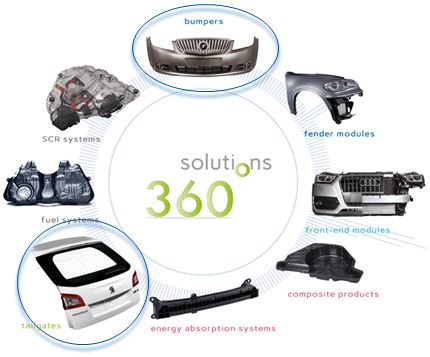
\includegraphics[scale=0.65]{image1-1}
    \end{column}
    \begin{column}{0.4\textwidth}
      SUV drag reduction study
      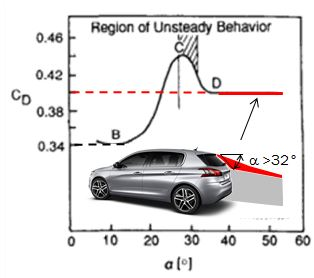
\includegraphics[scale=0.65]{image1-2}
    \end{column}
  \end{columns}
  \begin{columns}[onlytextwidth]
    \begin{column}{0.5\textwidth}
      Wind tunnel measurment and\\
      aerodynamic LES computations\\
      pressure coefficient : $C_p=\frac{P-P_\infty}{1/2pv^2}$
    \end{column}
    \begin{column}{0.5\textwidth}
      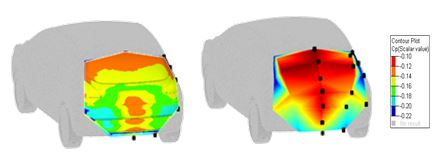
\includegraphics[scale=0.6]{image1-3} \\
      \quad computed $C_p$ \quad measured $C_p$
    \end{column}
  \end{columns}
\end{frame}

\begin{frame}{Plastic Omnium}
  Wake analysis on square back mock up :\\
  Frequency identification with cross-corelation and spectral coherency\\
  Phase average visualization at identified frequencies\\
  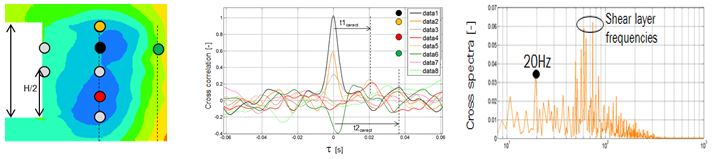
\includegraphics[scale=0.7]{image2-1}\\
  \quad \small Average $C_p$ \quad\quad\quad Spectral Coherency \quad\quad\quad Cross corelation\\
  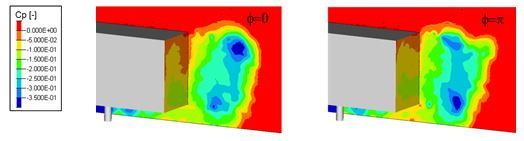
\includegraphics[scale=0.7]{image2-2}\\
  \quad\quad\quad\quad $C_p$ phase average at 20Hz\\
  High Number of time steps needed
\end{frame}

\section{Problem}
\begin{frame}<beamer>
  \frametitle{Contents}
  \tableofcontents[currentsection]
\end{frame}

\begin{frame}{Problem}
  \begin{block}{We are interested in the Navier-Stokes problem :}
    \[ \left\{
    \begin{aligned}
      &\frac{\partial\mathbf{v}}{\partial t} + (\mathbf{v}\cdot\grad)\mathbf{v} + \grad p + \frac{1}{Re}\laplace\mathbf{v} -f = 0\\
      &\div\mathbf{v} = 0\\
      &\mathbf{v}\big\rvert_{t=0} = \mathbf{v}_0
    \end{aligned}
    \right.\]
  \end{block}
  However Dirichlet boundary conditions can appear very restrictive, we would prefer more flexible boundary conditions.\\
  We'll use the curl formulation of Navier-Stokes.\\
  \[ \curl\mathbf{u} = \begin{pmatrix}
    \partial_y v_z - \partial_z v_y\\
    \partial_z v_x - \partial_x v_z\\
    \partial_x v_y - \partial_y v_x
  \end{pmatrix} \]
\end{frame}

\begin{frame}{Problem}
  \begin{block}{Curl formulation of Navier-Stokes Problem :}
    \begin{equation}
      \label{start}
      \left\{\begin{aligned}
      &\frac{\partial \mathbf{v}}{\partial t} + (\curl  \mathbf{v})\times \mathbf{v} + \grad q + \frac{1}{Re}\curll  \mathbf{v}-\mathbf{f} = 0\\
      &\div \mathbf{v} = 0\\
      &\mathbf{v}\big\rvert_{t=0} = \mathbf{v}_0
      \end{aligned}\right.
    \end{equation}
    where $q = \frac{|\mathbf{v}|^2}{2}+p$.
  \end{block}
  For generalized permeability boundary conditions, we need :
  \begin{align}
    &\mathbf{v}\cdot \mathbf{n}\restr = \alpha_0 \label{bc0}\\
    &(\curl  \mathbf{v})\cdot \mathbf{n}\restr = \alpha_1 \label{bc1}\\
    &(\curll  \mathbf{v})\cdot \mathbf{n}\restr = \alpha_2 \label{bc2}
  \end{align}
  \begin{itemize}
  \item (\ref{bc2}) is a boundary condition of order 2
  \item known normal component
  \item free tangential component
  \end{itemize}
\end{frame}

\begin{frame}{Problem}
  \begin{block}{Variables separation}
    We want to write the solution as
    \[ \sum_i c_i(t) \mathbf{g}_i(x,y,z) \]
    \begin{itemize}
    \item the coefficients $c_i$ handle the time dimension.
    \item the basis functions $(\mathbf{g}_i)$ handle the spatial dimension.
    \end{itemize}
  \end{block}
  Use of the works of P. Penel and J. Neustupa \cite{Penel2004} :
  \begin{itemize}
  \item $D^1(\Omega) = \{\mathbf{v} \in [H^1(\Omega)]^3\; |\; \div\mathbf{v}=0,\nabla^k\times \mathbf{v}\cdot \mathbf{n} = 0, k=0,1 \}$
  \item spanned by the eigen functions of the curl operator
  \item need to handle the boundary conditons apart (B. Surowiec)
  \end{itemize}
\end{frame}

\begin{frame}{Global Strategy}
  \centering
  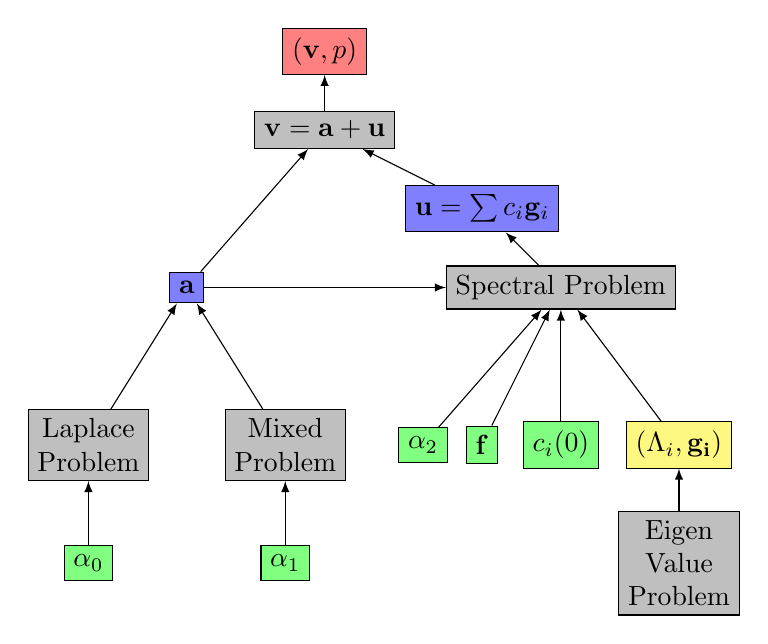
\begin{tikzpicture}
    \uncover<1-9>{\node[draw,fill=red!50] (v) at (3,-2) {$(\mathbf{v},p)$} ;}
    \uncover<2-9>{\node[draw,fill=gray!50] (pbv) at (3,-3) {$\mathbf{v}=\mathbf{a}+\mathbf{u}$} ;}
    \uncover<2-9>{\draw[->,>=latex] (pbv) -- (v);}
    \uncover<3-9>{\node[draw,fill=blue!50] (a) at (1.25,-5) {$\mathbf{a}$} ;}
    \uncover<3-9>{\draw[->,>=latex] (a) -- (pbv);}
    \uncover<4-9>{\node[draw,fill=gray!50,align=center] (pbpsi0) at (0,-7) {Laplace\\ Problem} ;}
    \uncover<4-9>{\draw[->,>=latex] (pbpsi0) -- (a);}
    \uncover<4-9>{\node[draw,fill=green!50] (alpha0) at (0,-8.5) {$\alpha_0$};}
    \uncover<4-9>{\draw[->,>=latex] (alpha0) -- (pbpsi0);}
    \uncover<5-9>{\node[draw,fill=gray!50,align=center] (pbcurlb) at (2.5,-7) {Mixed\\ Problem} ;}
    \uncover<5-9>{\draw[->,>=latex] (pbcurlb) -- (a);}
    \uncover<5-9>{\node[draw,fill=green!50] (alpha1) at (2.5,-8.5) {$\alpha_1$};}
    \uncover<5-9>{\draw[->,>=latex] (alpha1) -- (pbcurlb);}
    \uncover<6-9>{\node[draw,fill=blue!50] (u) at (5,-4) {$\mathbf{u}=\sum c_i\mathbf{g}_i$} ;}
    \uncover<6-9>{\draw[->,>=latex] (u) -- (pbv);}
    \uncover<6-9>{\node[draw,align=center,fill=gray!50] (pbc) at (6,-5) {Spectral Problem};}
    \uncover<6-9>{\draw[->,>=latex] (pbc) -- (u);}
    \uncover<7-9>{\draw[->,>=latex] (a) -- (pbc);}
    \uncover<8-9>{\node[draw,fill=green!50] (alpha2) at (4.25,-7) {$\alpha_2$};}
    \uncover<8-9>{\draw[->,>=latex] (alpha2) -- (pbc);}
    \uncover<8-9>{\node[draw,fill=green!50] (f) at (5,-7) {$\mathbf{f}$};}
    \uncover<8-9>{\draw[->,>=latex] (f) -- (pbc);}
    \uncover<8-9>{\node[draw,fill=green!50] (c0) at (6,-7) {$c_i(0)$};}
    \uncover<8-9>{\draw[->,>=latex] (c0) -- (pbc);}
    \uncover<9-9>{\node[draw,fill=yellow!50] (lambdagi) at (7.5,- 7) {$(\Lambda_i,\mathbf{g_i})$} ;}
    \uncover<9-9>{\draw[->,>=latex] (lambdagi) -- (pbc);}
    \uncover<9-9>{\node[draw,align=center,fill=gray!50] (pbeigen) at (7.5,-8.5) {Eigen\\ Value\\ Problem};}
    \uncover<9-9>{\draw[->,>=latex] (pbeigen) -- (lambdagi);}
  \end{tikzpicture}
\end{frame}

\section{Eigen Functions}
\begin{frame}<beamer>
  \frametitle{Contents}
  \begin{columns}[onlytextwidth]
    \begin{column}{0.35\textwidth}
      \tableofcontents[currentsection]
    \end{column}
    \begin{column}{0.65\textwidth}
      \centering
      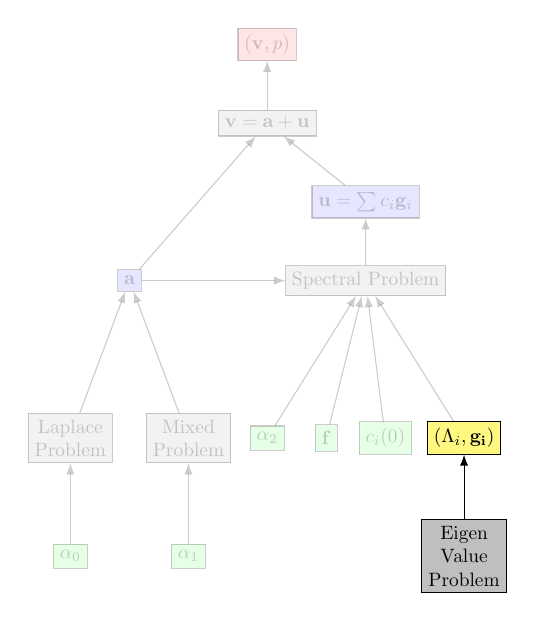
\begin{tikzpicture}
        \node[draw,scale=\tailleg,fill=red!50,opacity=0.2] (v) at (2.5,-2) {$(\mathbf{v},p)$} ;
        \node[draw,scale=\tailleg,fill=gray!50,opacity=0.2] (pbv) at (2.5,-3) {$\mathbf{v}=\mathbf{a}+\mathbf{u}$} ;
        \draw[->,>=latex,opacity=0.2] (pbv) -- (v);
        \node[draw,scale=\tailleg,fill=blue!50,opacity=0.2] (a) at (0.75,-5) {$\mathbf{a}$} ;
        \draw[->,>=latex,opacity=0.2] (a) -- (pbv);
        \node[draw,scale=\tailleg,fill=gray!50,align=center,opacity=0.2] (pbpsi0) at (0,-7) {Laplace\\ Problem} ;
        \draw[->,>=latex,opacity=0.2] (pbpsi0) -- (a);
        \node[draw,scale=\tailleg,fill=green!50,opacity=0.2] (alpha0) at (0,-8.5) {$\alpha_0$};
        \draw[->,>=latex,opacity=0.2] (alpha0) -- (pbpsi0);
        \node[draw,scale=\tailleg,fill=gray!50,align=center,opacity=0.2] (pbcurlb) at (1.5,-7) {Mixed\\ Problem} ;
        \draw[->,>=latex,opacity=0.2] (pbcurlb) -- (a);
        \node[draw,scale=\tailleg,fill=green!50,opacity=0.2] (alpha1) at (1.5,-8.5) {$\alpha_1$};
        \draw[->,>=latex,opacity=0.2] (alpha1) -- (pbcurlb);
        \node[draw,scale=\tailleg,fill=blue!50,opacity=0.2] (u) at (3.75,-4) {$\mathbf{u}=\sum c_i\mathbf{g}_i$} ;
        \draw[->,>=latex,opacity=0.2] (u) -- (pbv);
        \node[draw,scale=\tailleg,align=center,fill=gray!50,opacity=0.2] (pbc) at (3.75,-5) {Spectral Problem};
        \draw[->,>=latex,opacity=0.2] (pbc) -- (u);
        \draw[->,>=latex,opacity=0.2] (a) -- (pbc);
        \node[draw,scale=\tailleg,fill=green!50,opacity=0.2] (alpha2) at (2.5,-7) {$\alpha_2$};
        \draw[->,>=latex,opacity=0.2] (alpha2) -- (pbc);
        \node[draw,scale=\tailleg,fill=green!50,opacity=0.2] (f) at (3.25,-7) {$\mathbf{f}$};
        \draw[->,>=latex,opacity=0.2] (f) -- (pbc);
        \node[draw,scale=\tailleg,fill=green!50,opacity=0.2] (c0) at (4,-7) {$c_i(0)$};
        \draw[->,>=latex,opacity=0.2] (c0) -- (pbc);
        \node[draw,scale=\tailleg,fill=yellow!50] (lambdagi) at (5,- 7) {$(\Lambda_i,\mathbf{g_i})$} ;
        \draw[->,>=latex,opacity=0.2] (lambdagi) -- (pbc);
        \node[draw,scale=\tailleg,align=center,fill=gray!50] (pbeigen) at (5,-8.5) {Eigen\\ Value\\ Problem};
        \draw[->,>=latex] (pbeigen) -- (lambdagi);
      \end{tikzpicture}
    \end{column}
  \end{columns}
\end{frame}

\begin{frame}{$\mathbf{u}=\sum_{i=1}^\infty c_i\mathbf{g}_i$}
  We use the work of R. Rodriguez and P. Venegas \cite{Venegas2013} so we can compare and analyse our implementation.\\
  They studied the following problem on the sphere
  \begin{equation}\label{eigenStart}
    \left\{
    \begin{aligned}
      \curl\mathbf{g}&=\lambda\mathbf{g}\\
      \curl\mathbf{g}\cdot\mathbf{n}&=0
    \end{aligned}
    \right.
  \end{equation}
  Using the space $\Z=\{\mathbf{v}\in H(\mathrm{curl}) \quad|\quad \curl\mathbf{v}\cdot\mathbf{n} = 0 \mbox{ on } \Gamma\}$ this leads to :
  \begin{block}{Find $\lambda\in\R$ and $\mathbf{g}\in \Z$, $\mathbf{g}\neq 0$ such that}
    \begin{equation}\label{eigenwf}
      \int_\Omega \curl\mathbf{g}\cdot\curl\mathbf{v} = \lambda^2\int_\Omega \mathbf{g}\cdot\mathbf{v} \quad \forall\mathbf{v}\in \Z
    \end{equation}
  \end{block}
\end{frame}

\begin{frame}{$\mathbf{u}=\sum_{i=1}^\infty c_i\mathbf{g}_i$}
  In the event of the domain is symmetric, $\lambda$ and $-\lambda$ are eigen values, and $\mathbf{g}$ is not directly an eigen function of problem \ref{eigenStart}.\\
  It is a linear combination of the eigen functions associated to $\lambda$ and $-\lambda$.\\
  And the eigen space of $\mathbf{g}$ is the sum of the eigen spaces associated to $\lambda$ and $-\lambda$.
  \begin{block}{Discretization}
    Since $\Z\subset H(\mathrm{curl})$ we use Nedelec elements.\\
    \begin{align*}
      &\NN^k(T)=[\PP_{k-1}(T)]^3\oplus\{\mathbf{p}\in[\PP_k(T)]^3 \,|\,
      \mathbf{p(x)}\cdot\mathbf{x}=0 \}\\
      &\NN_h=\{\mathbf{v}_h\in H(\mathrm{curl};\Omega) \,|\,
      \mathbf{v}_h\restr{T}\in\NN^k(T)\, \forall T\in \TT_h \}\\
    \end{align*}
    We need to find a way to impose the boundary condition $\curl\mathbf{v}\cdot\mathbf{n}=0$.
  \end{block}
\end{frame}

\begin{frame}{$\mathbf{u}=\sum_{i=1}^\infty c_i\mathbf{g}_i$}
  According to V. Girault \cite{girault90-1}, we have that $\forall\mathbf{v}\in\Z$, $\mathbf{v}=\mathbf{w}+\grad q$ with $\mathbf{w}\in H(\mathrm{curl})$ and $\mathbf{w}\times\mathbf{n}=0$, and $q \in H^1(\Omega)$.\\
  Then, if we note
  \begin{itemize}
  \item $\{\bm{\phi}_i\}_{i=1}^M$, basis of $\NN_h(\Omega)$,
  \item $\{\bm{\phi}_i\}_{i=1}^N$, basis of $\NN_h(\Omega\setminus\Gamma)$,
  \item $\{\varphi_i\}_{i=1}^J$, basis of $\LLL_h(\Gamma)$,
  \end{itemize}
  and we choose one vertex on each connected component of $\Gamma=\cup_{i=0}^I\Gamma_i$, and assume that the corresponding functions are the last ones, then with $L=J-(I+1)$
  \begin{block}{A basis of $\Z_h$ is}
    \[ \{\bm{\phi}_i\}_{i=1}^N\cup\{\grad\varphi_i\}_{i=1}^L \]
  \end{block}
\end{frame}

\begin{frame}{$\mathbf{u}=\sum_{i=1}^\infty c_i\mathbf{g}_i$}
  We can write $\forall \mathbf{v}\in \Z_h \subset \NN_h$
  \[ \mathbf{v}=\underbrace{\sum_{m=1}^M\alpha_m\bm{\phi}_m}_{\NN_h}=\underbrace{\sum_{m=1}^N\alpha_m'\bm{\phi}_m+ \sum_{j=0}^L \beta_j\grad\varphi_j}_{\Z_h} \]
  and in the lowest order, if $e_m$ is the edge assiciated to the $m$-th dof,  we have :
  \[
  \alpha_m=\left\{\begin{aligned}
  &\alpha_m', &&\mbox{if } e_m\cap\Gamma = \emptyset,\\
  &\alpha_m'\pm \beta_j, &&\mbox{if } e_m\cap\Gamma = \{P_j\},\\
  &\alpha_m'\pm (\beta_j-\beta_k), &&\mbox{if } e_m\cap\Gamma = \{P_j,P_k\}
  (e_m\notin\Gamma),\\
  &\pm (\beta_j-\beta_k), &&\mbox{if } e_m=[P_j,P_k]\subset\Gamma
  \end{aligned}\right.
  \]
  With $\bm{\alpha}=(\alpha_1,\dots,\alpha_M)^t$ and $\widehat{\bm{\alpha}}=(\alpha_1',\dots,\alpha_M',\beta_1,\dots,\beta_J)^t$,\\
  there exists a matric $C$, of size $M\times(N+L)$ such that \[\bm{\alpha}=C\widehat{\bm{\alpha}} \]
\end{frame}

\begin{frame}[fragile]{Matric C}
  For all dof of $\NN_h$, we need to :
  \begin{itemize}
  \item find the associated edge, with the correct permutation,
    \begin{lstlisting}
auto const& eltLocalId = dof.first.elementId();
auto const& elt = mesh->element(eltLocalId);
auto const& edgeLocalId = dof.first.localDof();
auto perm = elt.edgePermutation( edgeLocalId );
    \end{lstlisting}
  \item find the vertex of the edge, with correct numbering,
    \begin{lstlisting}
auto i1 = elt.eToP(edgeLocalId, 0);
auto i2 = elt.eToP(edgeLocalId, 1);
auto const& pt1 = elt.point( i1 );
auto const& pt2 = elt.point( i2 );
    \end{lstlisting}
  \item find the position of the edge with respect to the boundary,
  \item remove one dof per connected component by using markers,
  \item create a matrix of size $M\times(M+K)$ and create the correct submatrix,
  \end{itemize}
\end{frame}

\begin{frame}{$\alpha=C\widehat{\alpha}$}
  \begin{itemize}
  \item $A=(\int_\Omega\curl\bm{\phi}_i\cdot\curl\bm{\phi}_j)_{ij}$, $B=(\int_\Omega\bm{\phi}_i\cdot\bm{\phi}_j)_{ij}$
  \item we use \texttt{PtAP} to create $\widehat{A}=C^tAC$, and $\widehat{B}=C^tBC$
  \end{itemize}
  
  \begin{figure}[H]
    \makebox[\textwidth][c]{
      \subfloat[spy $A$]{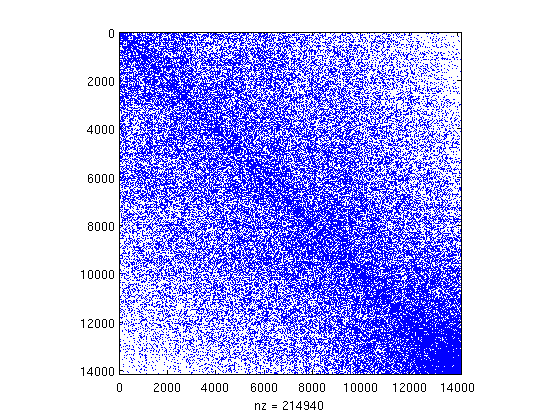
\includegraphics[scale=0.28]{spyA}}\ 
      \subfloat[spy $\widehat{A}$]{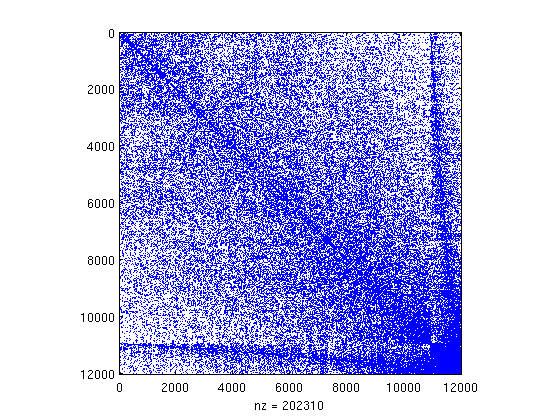
\includegraphics[scale=0.28]{spyAA}}
    }
  \end{figure}
  And then we use SLEPc to solve the following problem :
  \begin{block}{Solve the generalized hermitian eigen problem :}
    \begin{equation}\label{eigenhat}
      \widehat{A}\widehat{\bm{\alpha}}=\lambda \widehat{B}\widehat{\bm{\alpha}}
    \end{equation}
  \end{block}
\end{frame}

\begin{frame}{Results}
  \begin{figure}[H]
    \makebox[\textwidth][c]{
      \subfloat[mode 2]{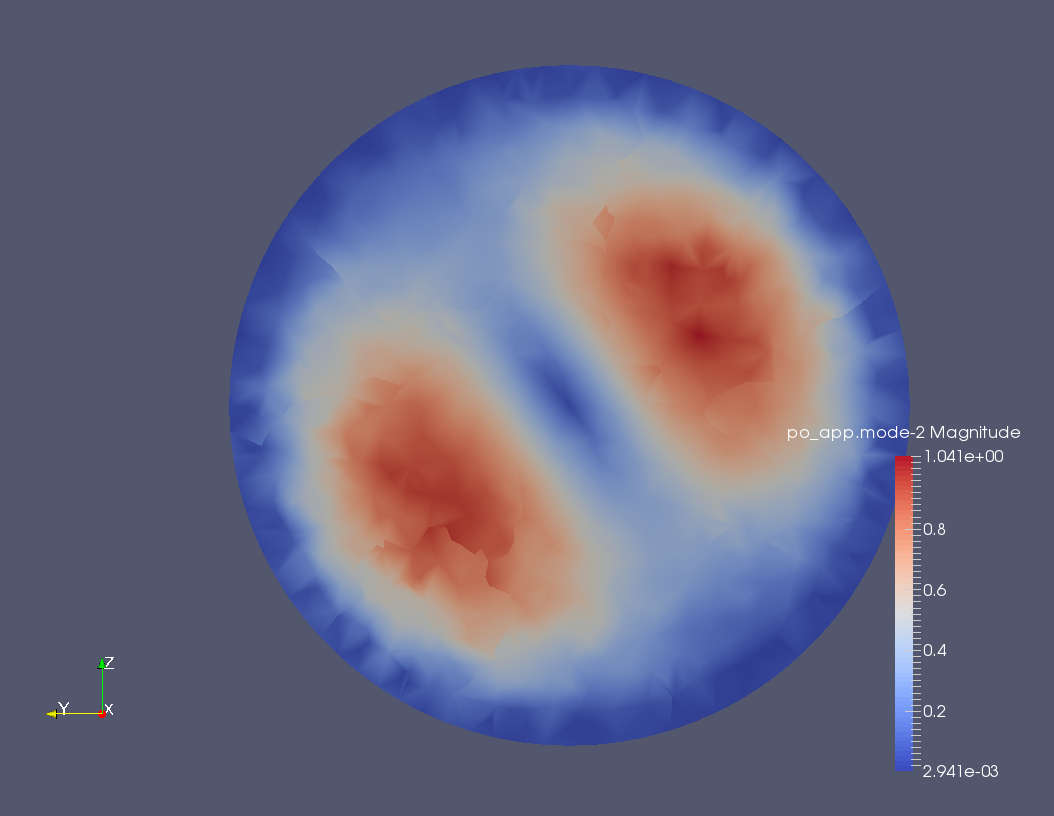
\includegraphics[scale=0.1]{mode2}}\ 
      \subfloat[mode 6]{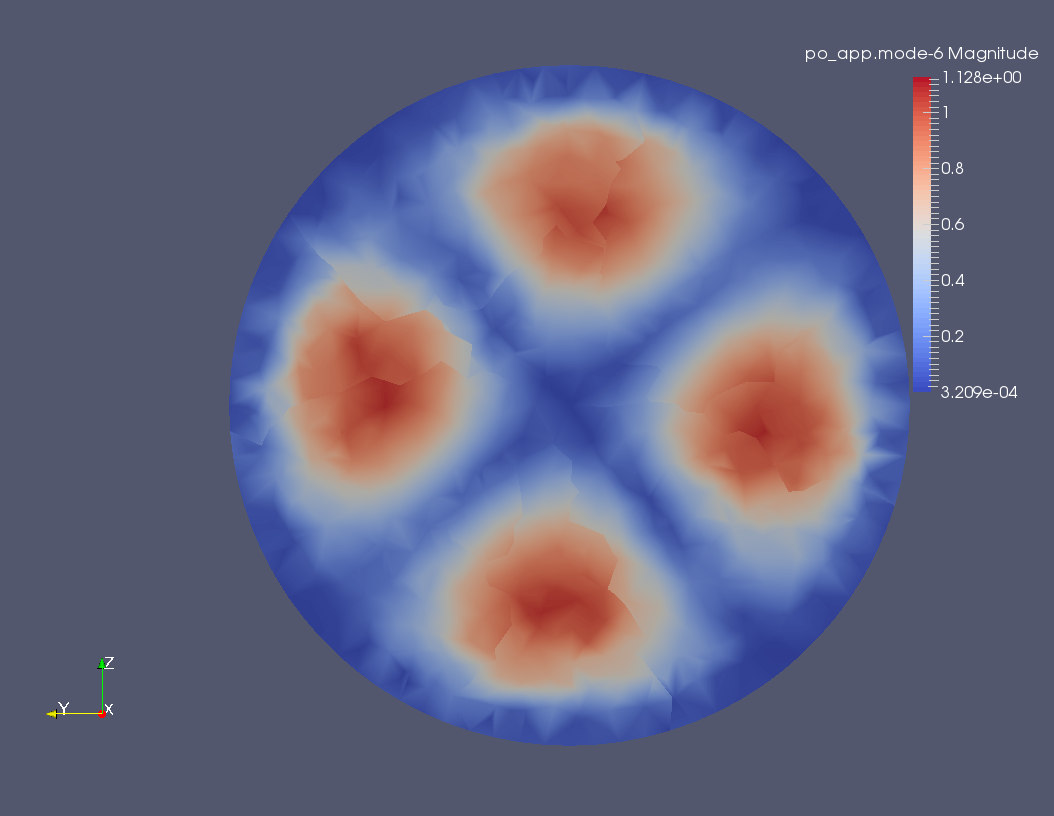
\includegraphics[scale=0.1]{mode6}}
    }
    \makebox[\textwidth][c]{
      \subfloat[mode 14]{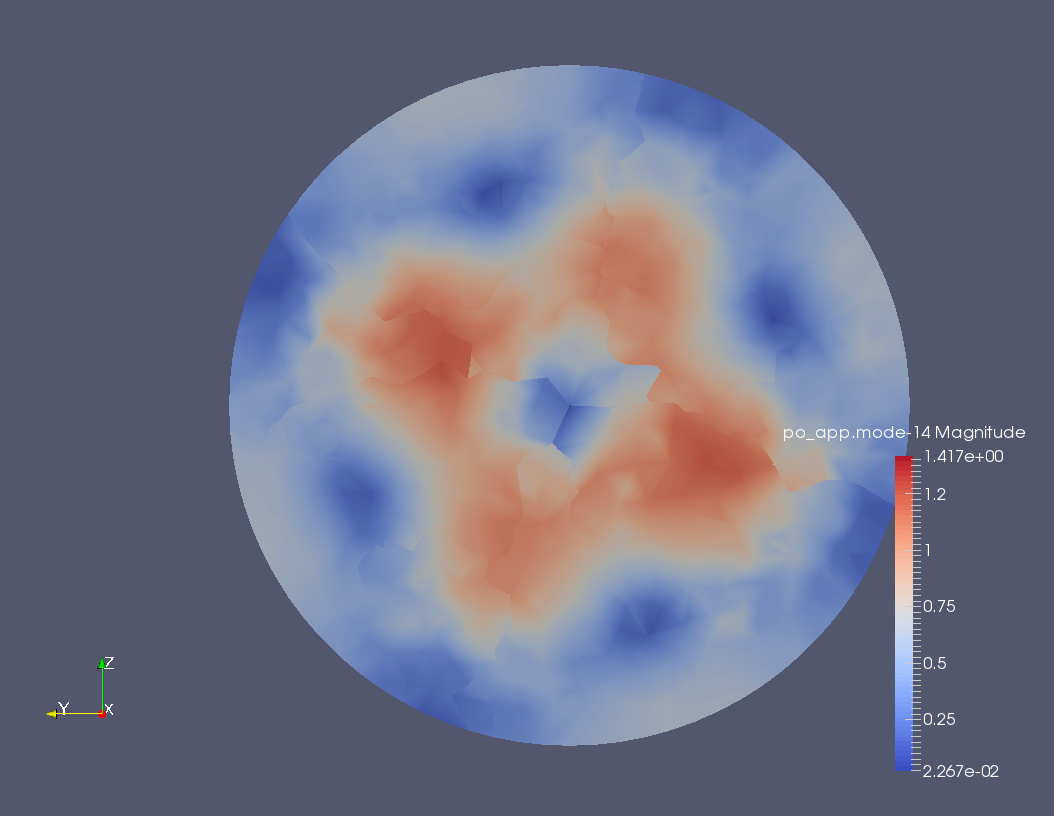
\includegraphics[scale=0.1]{mode14}}\ 
      \subfloat[mode 32]{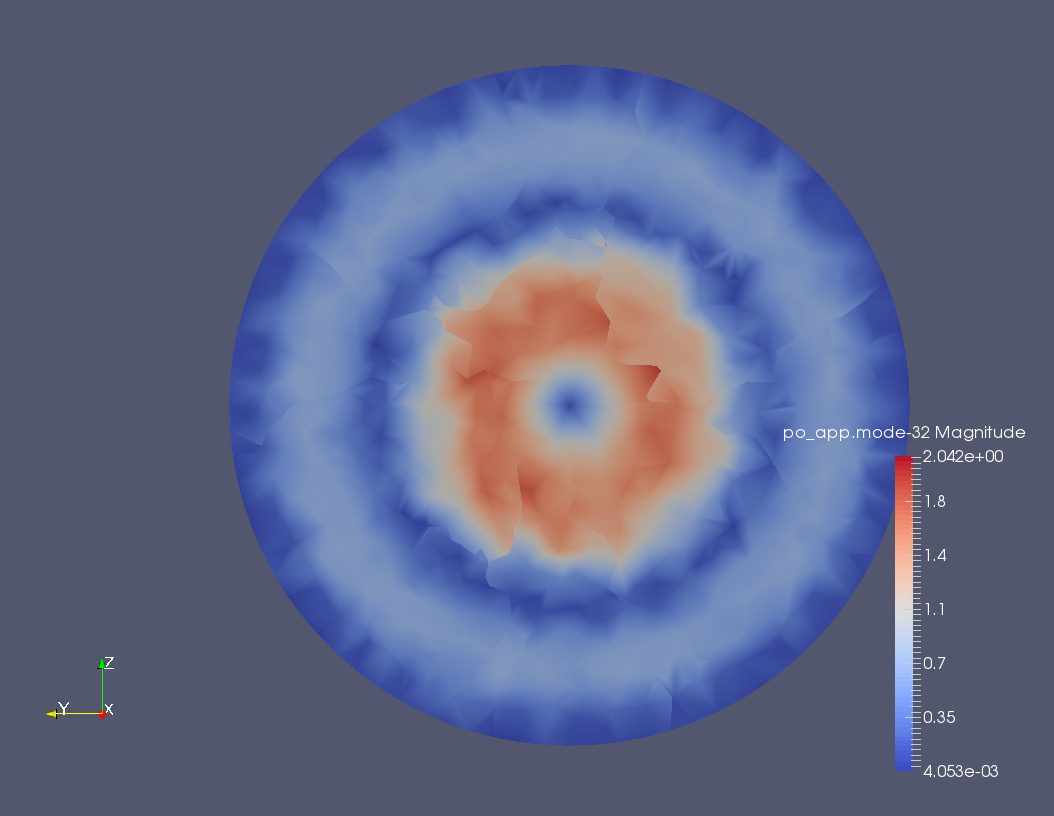
\includegraphics[scale=0.1]{mode32}}
    }
  \end{figure}
\end{frame}

\begin{frame}{Results}
  \begin{table}[H]
    \small
    \centering
    \begin{tabular}{r|c|c|c}
      h & 0.15 & 0.075 & 0.05 \\
      \# elements & 7000 & 50000 & 150000 \\
      \hline
      $\widehat{\lambda}_h$ & 4.49481924 & 4.49377347 & 4.49361\\
      $|\widehat{\lambda}_h-\lambda|$ & 0.00141024 & 0.00036447 & 0.000201 \\
      order & $-$ & 1.9521 & 1.4678 \\
      \hline
      $||\div\mathbf{u}||_2$ & 2.88311e-14 & 6.60701e-14 & 9.22039e-14 \\
      $||\mathbf{u}\cdot\mathbf{n}||_2$ & 0.216208 & 0.112487 & 0.0737108 \\
      $||\curl\mathbf{u}\cdot\mathbf{n}||_2$ & 5.11927e-15 & 9.48309e-15 & 1.47194e-14 \\
    \end{tabular}
  \end{table}
  \begin{columns}[onlytextwidth]
    \begin{column}{0.3\textwidth}
      Scalability for 50 modes :
    \end{column}
    \begin{column}{0.7\textwidth}
      \begin{figure}[H]
        \centering
        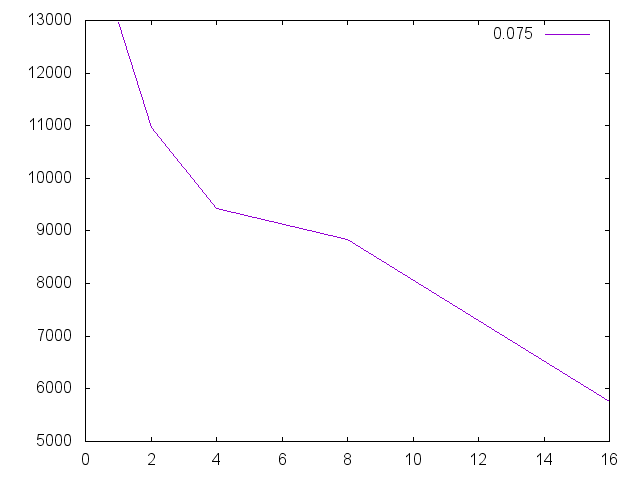
\includegraphics[scale=0.3]{eigen}
      \end{figure}
    \end{column}
  \end{columns}
\end{frame}

\section{Boundary conditions}
\begin{frame}<beamer>
  \frametitle{Contents}
  \begin{columns}[onlytextwidth]
    \begin{column}{0.35\textwidth}
      \tableofcontents[currentsection]
    \end{column}
    \begin{column}{0.65\textwidth}
      \centering
      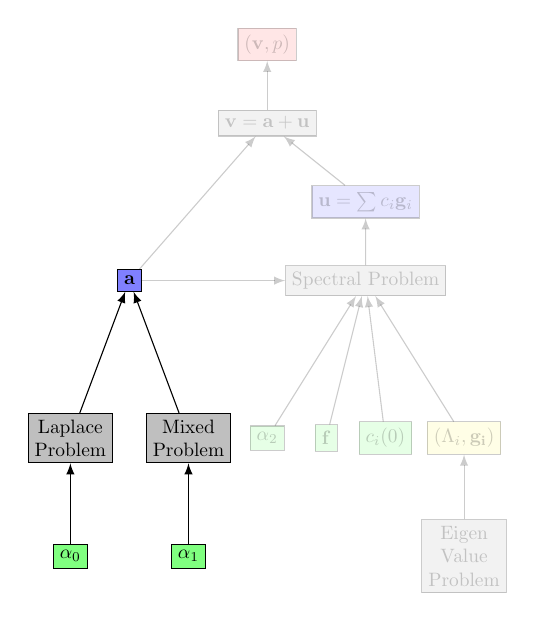
\begin{tikzpicture}
        \node[draw,scale=\tailleg,fill=red!50,opacity=0.2] (v) at (2.5,-2) {$(\mathbf{v},p)$} ;
        \node[draw,scale=\tailleg,fill=gray!50,opacity=0.2] (pbv) at (2.5,-3) {$\mathbf{v}=\mathbf{a}+\mathbf{u}$} ;
        \draw[->,>=latex,opacity=0.2] (pbv) -- (v);
        \node[draw,scale=\tailleg,fill=blue!50] (a) at (0.75,-5) {$\mathbf{a}$} ;
        \draw[->,>=latex,opacity=0.2] (a) -- (pbv);
        \node[draw,scale=\tailleg,fill=gray!50,align=center] (pbpsi0) at (0,-7) {Laplace\\ Problem} ;
        \draw[->,>=latex] (pbpsi0) -- (a);
        \node[draw,scale=\tailleg,fill=green!50] (alpha0) at (0,-8.5) {$\alpha_0$};
        \draw[->,>=latex] (alpha0) -- (pbpsi0);
        \node[draw,scale=\tailleg,fill=gray!50,align=center] (pbcurlb) at (1.5,-7) {Mixed\\ Problem} ;
        \draw[->,>=latex] (pbcurlb) -- (a);
        \node[draw,scale=\tailleg,fill=green!50] (alpha1) at (1.5,-8.5) {$\alpha_1$};
        \draw[->,>=latex] (alpha1) -- (pbcurlb);
        \node[draw,scale=\tailleg,fill=blue!50,opacity=0.2] (u) at (3.75,-4) {$\mathbf{u}=\sum c_i\mathbf{g}_i$} ;
        \draw[->,>=latex,opacity=0.2] (u) -- (pbv);
        \node[draw,scale=\tailleg,align=center,fill=gray!50,opacity=0.2] (pbc) at (3.75,-5) {Spectral Problem};
        \draw[->,>=latex,opacity=0.2] (pbc) -- (u);
        \draw[->,>=latex,opacity=0.2] (a) -- (pbc);
        \node[draw,scale=\tailleg,fill=green!50,opacity=0.2] (alpha2) at (2.5,-7) {$\alpha_2$};
        \draw[->,>=latex,opacity=0.2] (alpha2) -- (pbc);
        \node[draw,scale=\tailleg,fill=green!50,opacity=0.2] (f) at (3.25,-7) {$\mathbf{f}$};
        \draw[->,>=latex,opacity=0.2] (f) -- (pbc);
        \node[draw,scale=\tailleg,fill=green!50,opacity=0.2] (c0) at (4,-7) {$c_i(0)$};
        \draw[->,>=latex,opacity=0.2] (c0) -- (pbc);
        \node[draw,scale=\tailleg,fill=yellow!50,opacity=0.2] (lambdagi) at (5,- 7) {$(\Lambda_i,\mathbf{g_i})$} ;
        \draw[->,>=latex,opacity=0.2] (lambdagi) -- (pbc);
        \node[draw,scale=\tailleg,align=center,fill=gray!50,opacity=0.2] (pbeigen) at (5,-8.5) {Eigen\\ Value\\ Problem};
        \draw[->,>=latex,opacity=0.2] (pbeigen) -- (lambdagi);
      \end{tikzpicture}
    \end{column}
  \end{columns}
\end{frame}

\begin{frame}{Boundary conditions}
  \label{psi0}
  \begin{block}{Decomposition of $\mathbf{a}$}
    \begin{center}
      \begin{tabular}{c|ccccc}
        & $\mathbf{a}$ & = & $\grad\psi^0$ & + & $\curl \mathbf{b}$ \\ \hline
        $\div\star$ & 0 & & $\laplace\psi^0$ & & 0\\ \hline
        $\star\cdot \mathbf{n}\restr$ & $\alpha_0$ & & $\alpha_0$ & & 0\\ \hline
        $\curl\star\cdot \mathbf{n}\restr$ & $\alpha_1$ & & 0 & & $\alpha_1$
      \end{tabular}
    \end{center}
  \end{block}
  2 choices to handle $\alpha_0$ by $\grad\psi^0$ :
  \begin{itemize}
  \item Laplacian in $H^1$
  \item Mixed problem in $H(\mathrm{div})$
  \end{itemize}
  2 choices to handle $\alpha_1$ by $\curl\mathbf{b}$ :
  \begin{itemize}
  \item Mixed problem in $H(\mathrm{curl})$
  \item using the basis $(\mathbf{g}_i)$ in $D^1$
  \end{itemize}
\end{frame}

\begin{frame}{Example}
  \begin{center}
  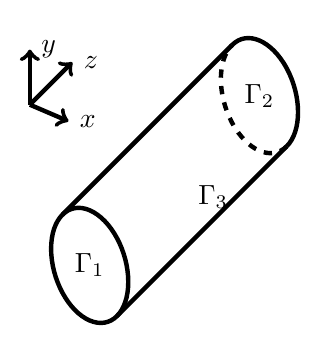
\begin{tikzpicture}
    \begin{scope}[x={(.7cm,-.3cm)}]
      \path (1,0,0);
      \pgfgetlastxy{\cylxx}{\cylxy}
      \path (0,1,0);
      \pgfgetlastxy{\cylyx}{\cylyy}
      \path (0,0,1);
      \pgfgetlastxy{\cylzx}{\cylzy}
      \pgfmathsetmacro{\cylt}{(\cylzy * \cylyx - \cylzx * \cylyy)/ (\cylzy * \cylxx - \cylzx * \cylxy)}
      \pgfmathsetmacro{\ang}{atan(\cylt)}
      \pgfmathsetmacro{\ct}{1/sqrt(1 + (\cylt)^2)}
      \pgfmathsetmacro{\st}{\cylt * \ct}
      \begin{scope}[every path/.style={ultra thick}]
        \draw[scale=0.7] (0,0,0) circle[radius=1];
        \draw[->,scale=0.7] (-1,3,1) -- (0,3,1);
        \draw[scale=0.7] (0,3,1) node [right] {$x$};
        \draw[->,scale=0.7] (-1,3,1) -- (-1,4,1);
        \draw[scale=0.7] (-1,4,1) node [right] {$y$};
        \draw[->,scale=0.7] (-1,3,1) -- (-1,3,-1);
        \draw[scale=0.7] (-1,3,-1) node [right] {$z$};
        \draw[scale=0.7] (\ct,\st,0) -- ++(0,0,-8);
        \draw[scale=0.7] (-\ct,-\st,0) -- ++(0,0,-8);
        \draw[scale=0.7] (\ct,\st,-8) arc[start angle=\ang,delta angle=180,radius=1];
        \draw[dashed,scale=0.7] (\ct,\st,-8) arc[start angle=\ang,delta angle=-180,radius=1];
        \draw[scale=0.7] (0,0,0) node {$\Gamma_1$};
        \draw[scale=0.7] (0,0,-8) node {$\Gamma_2$};
        \draw[scale=0.7] (1,0,-4) node {$\Gamma_3$};
      \end{scope}
    \end{scope}
  \end{tikzpicture}
  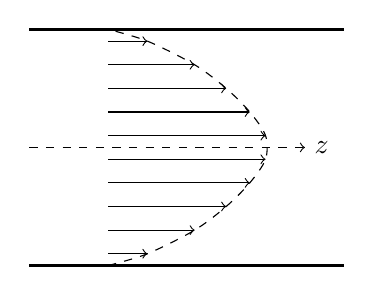
\begin{tikzpicture}
    \draw[very thick] (0,0) -- (4,0) ;
    \draw[dashed] plot[smooth] coordinates{(1,0)(1.5,0.15)(2.1,0.45)(2.5,0.75)(2.8,1.05)(3,1.35)(3,1.65)(2.8,1.95)(2.5,2.25)(2.1,2.55)(1.5,2.85)(1,3)} ;
    \draw[->] (1,0.15) -- (1.5,0.15) ;
    \draw[->] (1,0.45) -- (2.1,0.45) ;
    \draw[->] (1,0.75) -- (2.5,0.75) ;
    \draw[->] (1,1.05) -- (2.8,1.05) ;
    \draw[->] (1,1.35) -- (3,1.35) ;
    \draw[->, dashed] (0,1.5) -- (3.5,1.5) node[right] {$z$} ;
    \draw[->] (1,1.65) -- (3,1.65) ;
    \draw[->] (1,1.95) -- (2.8,1.95) ;
    \draw[->] (1,2.25) -- (2.5,2.25) ;
    \draw[->] (1,2.55) -- (2.1,2.55) ;
    \draw[->] (1,2.85) -- (1.5,2.85) ;
    \draw[very thick] (0,3) -- (4,3) ;
  \end{tikzpicture}
  \end{center}
  \[
  R=0.5,\ v=1\quad
  n\big\rvert_{\Gamma_1} =
  \begin{pmatrix}
    0\\0\\-1
  \end{pmatrix}
  n\big\rvert_{\Gamma_2} =
  \begin{pmatrix}
    0\\0\\1
  \end{pmatrix}
  n\big\rvert_{\Gamma_3} =
  \begin{pmatrix}
    x/R\\y/R\\0
  \end{pmatrix}
  \]
  \[
  \alpha_0 =
  \begin{cases}
    -2v\left(1-\frac{x^2+y^2}{R^2}\right)\\2v\left(1-\frac{x^2+y^2}{R^2}\right)\\0
  \end{cases}
  \alpha_1 =
  \begin{cases}
    0\\0\\0
  \end{cases}
  \alpha_2 =
  \begin{cases}
    -8v/R^2 & \mbox{ on } \Gamma_1\\
    8v/R^2 & \mbox{ on } \Gamma_2\\
    0 & \mbox{ on } \Gamma_3
  \end{cases}
  \]
\end{frame}

\begin{frame}{Results}
  \centering
  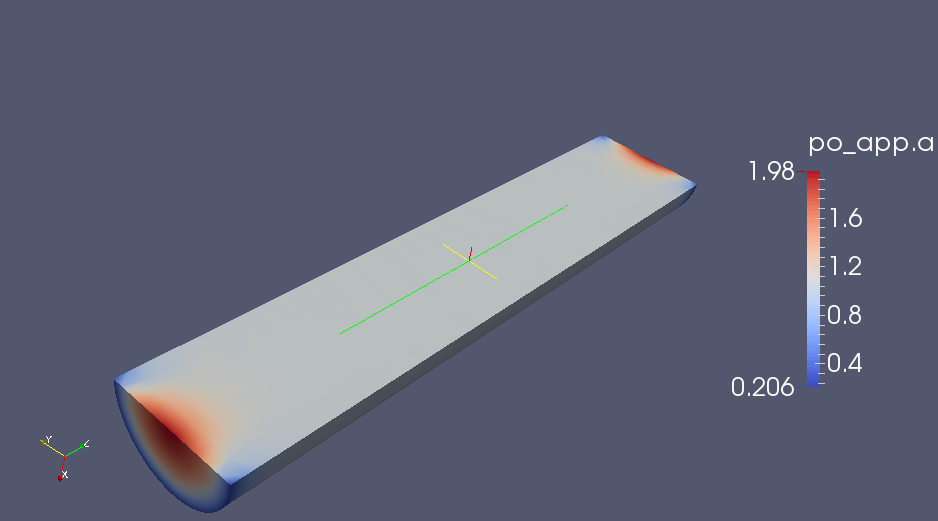
\includegraphics[scale=0.2]{psi0-clip}
  \begin{figure}[H]
	\makebox[\textwidth][c]{
	  \subfloat[inflow]{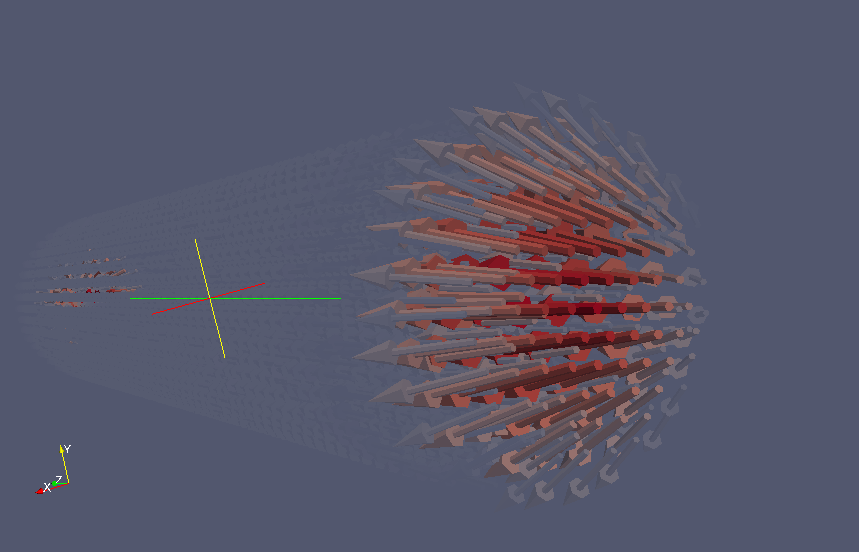
\includegraphics[scale=0.15]{aIn}}\ 
	  \subfloat[outflow]{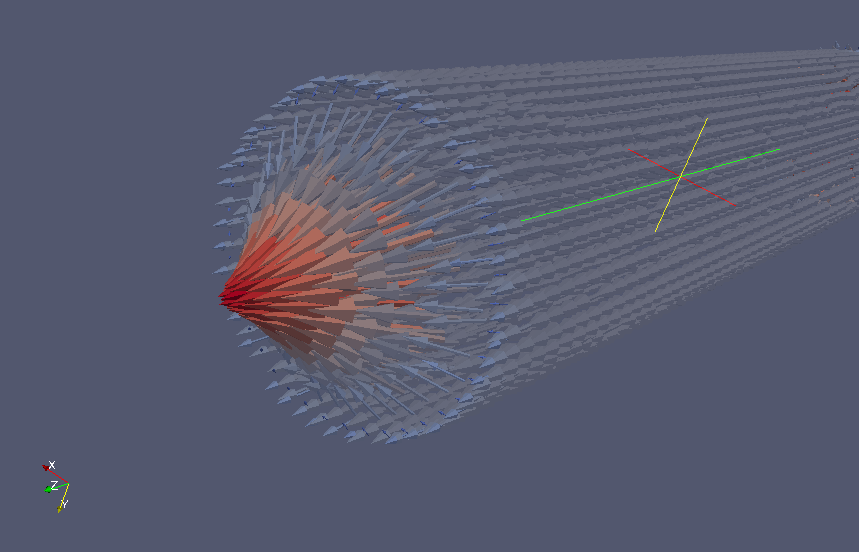
\includegraphics[scale=0.15]{aOut}}
	}
  \end{figure}
\end{frame}

\section{Spectral Problem}
\begin{frame}<beamer>
  \frametitle{Contents}
  \begin{columns}[onlytextwidth]
    \begin{column}{0.35\textwidth}
      \tableofcontents[currentsection]
    \end{column}
    \begin{column}{0.65\textwidth}
      \centering
      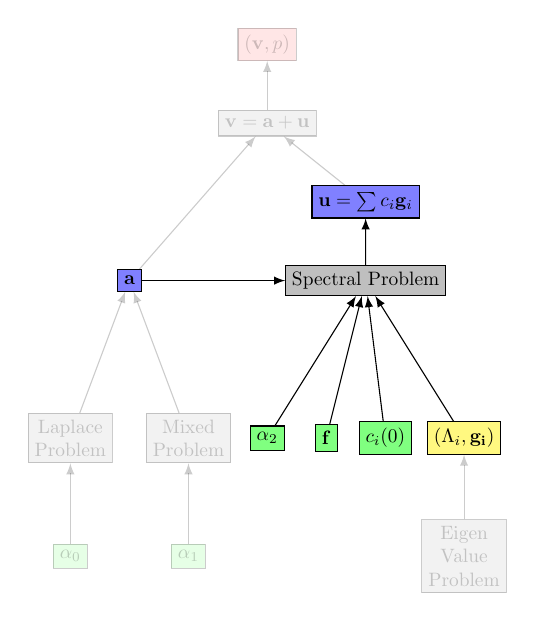
\begin{tikzpicture}
        \node[draw,scale=\tailleg,fill=red!50,opacity=0.2] (v) at (2.5,-2) {$(\mathbf{v},p)$} ;
        \node[draw,scale=\tailleg,fill=gray!50,opacity=0.2] (pbv) at (2.5,-3) {$\mathbf{v}=\mathbf{a}+\mathbf{u}$} ;
        \draw[->,>=latex,opacity=0.2] (pbv) -- (v);
        \node[draw,scale=\tailleg,fill=blue!50] (a) at (0.75,-5) {$\mathbf{a}$} ;
        \draw[->,>=latex,opacity=0.2] (a) -- (pbv);
        \node[draw,scale=\tailleg,fill=gray!50,align=center,opacity=0.2] (pbpsi0) at (0,-7) {Laplace\\ Problem} ;
        \draw[->,>=latex,opacity=0.2] (pbpsi0) -- (a);
        \node[draw,scale=\tailleg,fill=green!50,opacity=0.2] (alpha0) at (0,-8.5) {$\alpha_0$};
        \draw[->,>=latex,opacity=0.2] (alpha0) -- (pbpsi0);
        \node[draw,scale=\tailleg,fill=gray!50,align=center,opacity=0.2] (pbcurlb) at (1.5,-7) {Mixed\\ Problem} ;
        \draw[->,>=latex,opacity=0.2] (pbcurlb) -- (a);
        \node[draw,scale=\tailleg,fill=green!50,opacity=0.2] (alpha1) at (1.5,-8.5) {$\alpha_1$};
        \draw[->,>=latex,opacity=0.2] (alpha1) -- (pbcurlb);
        \node[draw,scale=\tailleg,fill=blue!50] (u) at (3.75,-4) {$\mathbf{u}=\sum c_i\mathbf{g}_i$} ;
        \draw[->,>=latex,opacity=0.2] (u) -- (pbv);
        \node[draw,scale=\tailleg,align=center,fill=gray!50] (pbc) at (3.75,-5) {Spectral Problem};
        \draw[->,>=latex] (pbc) -- (u);
        \draw[->,>=latex] (a) -- (pbc);
        \node[draw,scale=\tailleg,fill=green!50] (alpha2) at (2.5,-7) {$\alpha_2$};
        \draw[->,>=latex] (alpha2) -- (pbc);
        \node[draw,scale=\tailleg,fill=green!50] (f) at (3.25,-7) {$\mathbf{f}$};
        \draw[->,>=latex] (f) -- (pbc);
        \node[draw,scale=\tailleg,fill=green!50] (c0) at (4,-7) {$c_i(0)$};
        \draw[->,>=latex] (c0) -- (pbc);
        \node[draw,scale=\tailleg,fill=yellow!50] (lambdagi) at (5,- 7) {$(\Lambda_i,\mathbf{g_i})$} ;
        \draw[->,>=latex] (lambdagi) -- (pbc);
        \node[draw,scale=\tailleg,align=center,fill=gray!50,opacity=0.2] (pbeigen) at (5,-8.5) {Eigen\\ Value\\ Problem};
        \draw[->,>=latex,opacity=0.2] (pbeigen) -- (lambdagi);
      \end{tikzpicture}
    \end{column}
  \end{columns}
\end{frame}

\begin{frame}{Spectral Problem}
  Considering the solution $\mathbf{v}=\mathbf{u}+\mathbf{a}$ in (\ref{start}), we get :
  \begin{align*}
    \frac{\partial \mathbf{u}}{\partial t} &+ (\curl \mathbf{u})\times \mathbf{u} + (\curl \mathbf{u})\times \mathbf{a} + \left(\curl \mathbf{a}\right)\times \mathbf{u} \\
    &+ \grad\pi_\mathbf{a} + \frac{1}{Re}\curll \mathbf{u} - \mathbf{f_a} = 0
  \end{align*}
  where : $\pi_a=\frac{|\mathbf{u}+\mathbf{a}|^2}{2}$ and $\mathbf{f_a}=\mathbf{f}-\frac{\partial \mathbf{a}}{\partial t}-(\curl\mathbf{a})\times\mathbf{a}$.
  \begin{block}{Find $\mathbf{u}\in D^1$ such that $\forall \bm{\varphi}=\bm{\varphi}_0+\grad\phi\in D^1$ :}
    \begin{align*}
      \int_\Omega \frac{\partial \mathbf{u}}{\partial t}\cdot \bm{\varphi} &+ \int_\Omega ((\curl \mathbf{u})\times \mathbf{u})\cdot \bm{\varphi} + \int_\Omega ((\curl \mathbf{u})\times \mathbf{a})\cdot\bm{\varphi} \\
      &+ \int_\Omega ((\curl \mathbf{a})\times \mathbf{u})\cdot\bm{\varphi} + \frac{1}{Re}\int_\Omega (\curl \mathbf{u})\cdot(\curl\bm{\varphi}) \\
      &-\frac{1}{Re}\int_{\partial\Omega} \alpha_2\phi = \int_\Omega \mathbf{f_a}\cdot\bm{\varphi}
    \end{align*}
  \end{block}
\end{frame}

\begin{frame}{Discretization}
  By using $\mathbf{u}_M(x,y,z,t)=\sum_{i=1}^M c_i(t)\mathbf{g}_i(x,y,z)$ and by noting :
  \begin{align*}
    R_{ijk} &= \int_\Omega((\curl\mathbf{g_i})\times \mathbf{g_j})\cdot\mathbf{g_k} & R_{iak} &= \int_\Omega((\curl\mathbf{g_i})\times \mathbf{a})\cdot\mathbf{g_k}\\
    R_{iak} &= \int_\Omega((\curl\mathbf{a})\times \mathbf{g_i})\cdot\mathbf{g_k} & R_{fk} &= \int_\Omega\mathbf{f_a}\cdot\mathbf{g_k}\\
    R_{pk} &= \int_{\partial\Omega} \alpha_2\phi_k
  \end{align*}

  We use the Eigen library to solve the following problem :
  \begin{block}{Find $(c_i)_{i=1,\dots,M}$ such that $\forall k=1,\dots,M$ :}
    \[ \frac{\partial {\color{red}c_k}}{\partial t} + \frac{1}{Re}{\color{red}c_k}\lambda_k^2 + \sum_{i,j=1}^M{\color{red}c_ic_j}{\color{green}R_{ijk}} + \sum_{i=1}^M{\color{red}c_i}\left({\color{green}R_{iak}} + {\color{green}R_{iak}}\right) = {\color{green}R_{fk}} + \frac{1}{Re}{\color{green}R_{pk}} \]
  \end{block}
  where {\color{red} $c$} depends only on the time, and {\color{green} $R$} depends only on the space.
\end{frame}

\begin{frame}{Results}
  \begin{figure}[H]
	\makebox[\textwidth][c]{
      \subfloat{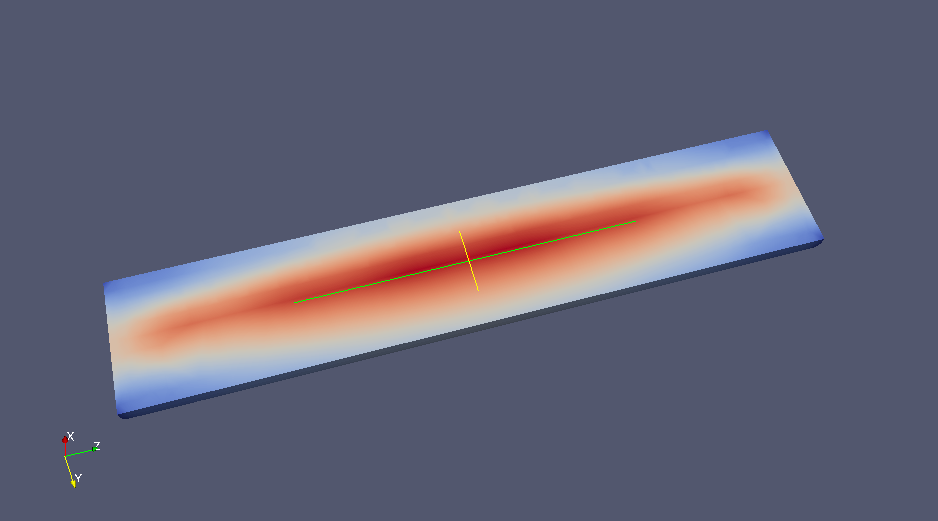
\includegraphics[scale=0.15,trim=0mm 20mm 0mm 20mm,clip]{v100modes}}\ 
	  \subfloat{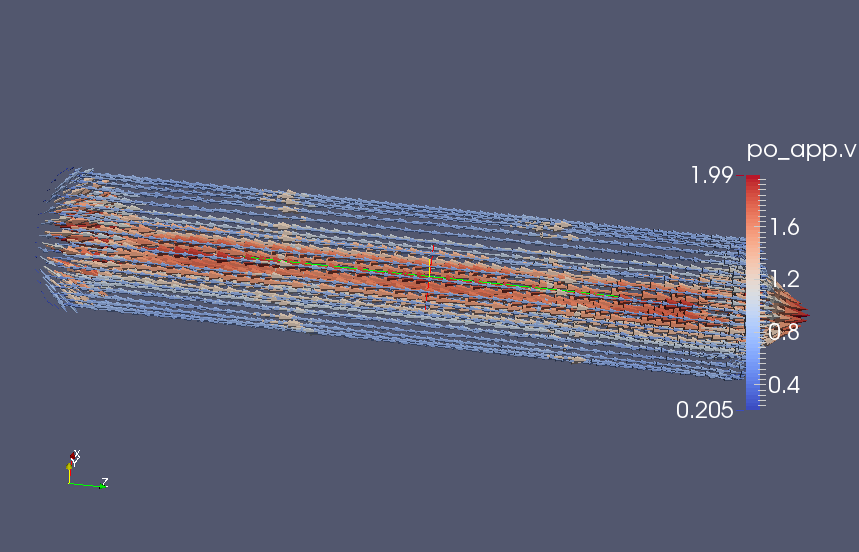
\includegraphics[scale=0.15,trim=0mm 20mm 0mm 30mm,clip]{vGradPression32-32}}
	}
    \caption{M = 50}
  \end{figure}
  \begin{figure}[H]
	\makebox[\textwidth][c]{
      \subfloat[M=10]{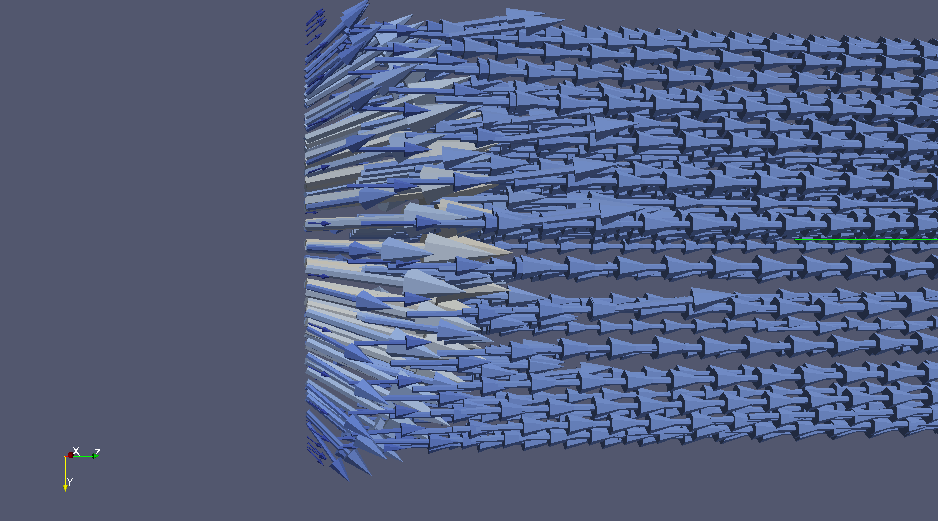
\includegraphics[scale=0.25,trim=100mm 20mm 100mm 20mm,clip]{vIn10}}\ 
	  \subfloat[M=100]{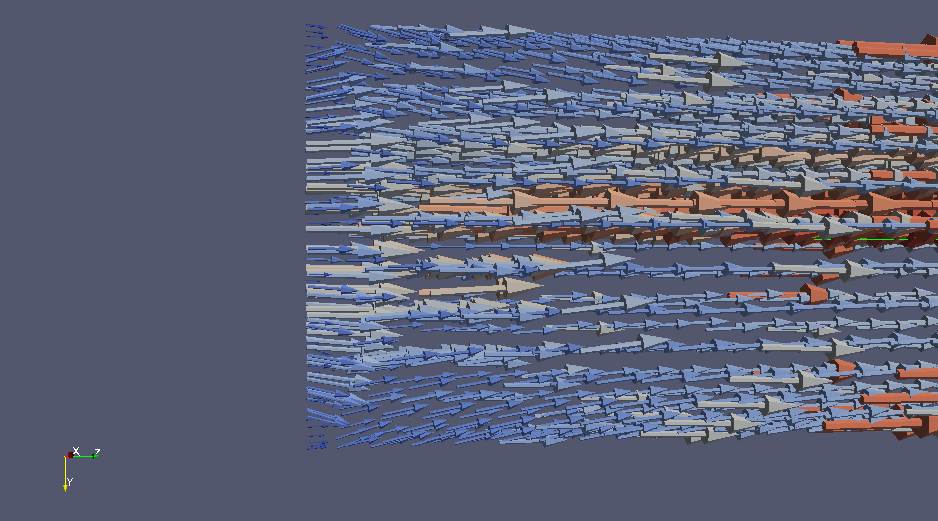
\includegraphics[scale=0.25,trim=100mm 20mm 100mm 20mm,clip]{vIn100}}
	}
  \end{figure}
\end{frame}

\section{Conclusion}
\begin{frame}<beamer>
  \frametitle{Contents}
  \tableofcontents[currentsection]
\end{frame}

\begin{frame}
  \centering
  \begin{tikzpicture}
    \node[draw,fill=red!50] (v) at (3,2) {$(\mathbf{v},p)$} ;
    \node (vIm) at (0,2) {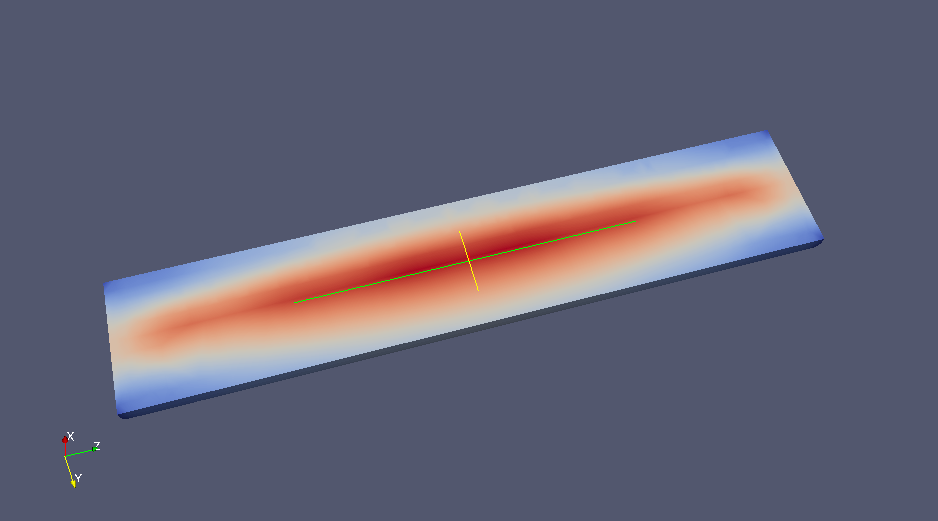
\includegraphics[scale=0.1,trim=0mm 30mm 20mm 30mm,clip]{v100modes}} ;
    \node[draw,fill=gray!50] (pbv) at (3,3) {$\mathbf{v}=\mathbf{a}+\mathbf{u}$} ;
    \draw[->,>=latex] (pbv) -- (v);
    \node[draw,fill=blue!50] (a) at (1.25,5) {$\mathbf{a}$} ;
    \node (psi0Im) at (0,5) {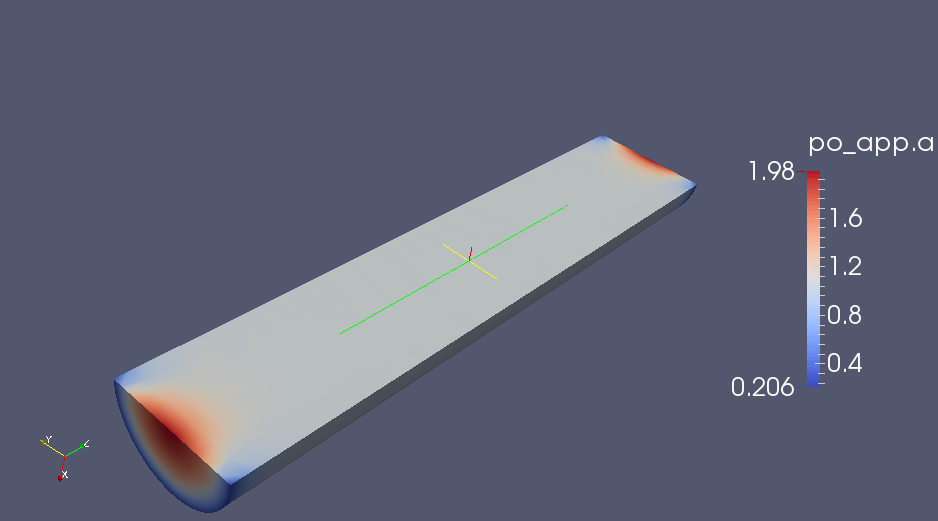
\includegraphics[scale=0.1,angle=90,trim=35mm 0mm 80mm 0mm,clip]{psi0-clip}} ;
    \draw[->,>=latex] (a) -- (pbv);
    \node[draw,fill=gray!50,align=center] (pbpsi0) at (0,7) {Laplace\\ Problem} ;
    \draw[->,>=latex] (pbpsi0) -- (a);
    \node[draw,fill=green!50] (alpha0) at (0,8.5) {$\alpha_0$};
    \draw[->,>=latex] (alpha0) -- (pbpsi0);
    \node[draw,fill=gray!50,align=center] (pbcurlb) at (2.5,7) {Mixed\\ Problem} ;
    \draw[->,>=latex] (pbcurlb) -- (a);
    \node[draw,fill=green!50] (alpha1) at (2.5,8.5) {$\alpha_1$};
    \draw[->,>=latex] (alpha1) -- (pbcurlb);
    \node[draw,fill=blue!50] (u) at (5,4) {$\mathbf{u}=\sum c_i\mathbf{g}_i$} ;
    \node (uIm) at (5.75,2.75) {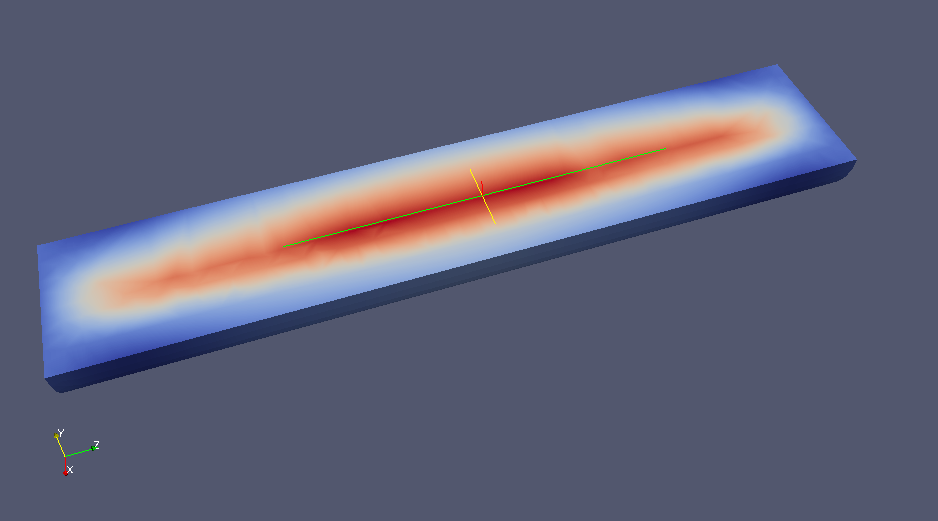
\includegraphics[scale=0.1,trim=0mm 40mm 20mm 15mm,clip]{u-clip}} ;
    \draw[->,>=latex] (u) -- (pbv);
    \node[draw,align=center,fill=gray!50] (pbc) at (6,5) {Spectral Problem};
    \draw[->,>=latex] (pbc) -- (u);
    \draw[->,>=latex] (a) -- (pbc);
    \node[draw,fill=green!50] (alpha2) at (4.25,7) {$\alpha_2$};
    \draw[->,>=latex] (alpha2) -- (pbc);
    \node[draw,fill=green!50] (f) at (5,7) {$\mathbf{f}$};
    \draw[->,>=latex] (f) -- (pbc);
    \node[draw,fill=green!50] (c0) at (6,7) {$c_i(0)$};
    \draw[->,>=latex] (c0) -- (pbc);
    \node[draw,fill=yellow!50] (lambdagi) at (7.5, 7) {$(\Lambda_i,\mathbf{g_i})$} ;
    \draw[->,>=latex] (lambdagi) -- (pbc);
    \node[draw,align=center,fill=gray!50] (pbeigen) at (7.5,8.5) {Eigen\\ Value\\ Problem};
    \draw[->,>=latex] (pbeigen) -- (lambdagi);
  \end{tikzpicture}
\end{frame}

\begin{frame}{Computing time}
  \centering
  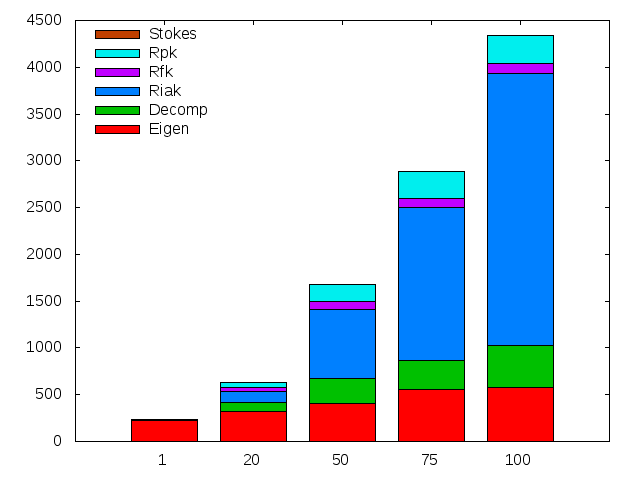
\includegraphics[scale=0.6]{histo}
\end{frame}

\begin{frame}{Perspectives}
  \begin{itemize}
  \item Improve SLEPc interface
  \item Tests intensively
    \begin{itemize}
    \item scalability
    \item max capacity
    \end{itemize}
  \item Use of conforming elements ($\Z_h$)
  \item Improve the framework
    \begin{itemize}
    \item decomposition using $\beta_j$
    \item handle $\alpha_2$ apart
    \item choices of problems for $\alpha_i$
    \end{itemize}
  \item Work on Plastic Omnium geometries 
  \end{itemize}
\end{frame}

\begin{frame}
  \begin{center}
    Thanks !
  \end{center}
\end{frame}

\begin{frame}[allowframebreaks]
  \frametitle<presentation>{Further Reading}
  \begin{thebibliography}{10}
    \beamertemplatebookbibitems
  \bibitem{girault90-1}
    V.~Girault.
    \newblock Curl-conforming finite element methods for Navier-Stokes equations with non-standard boundary conditions in $R^3$.
    \newblock {\em The Navier-Stokes Equations Theory and Numerical Methods}, volume 1431 of {\em Lecture Notes in Mathematics}, 1990.
    \beamertemplatearticlebibitems
  \bibitem{Penel2004}
    Bellout, Hamid and Neustupa, Jiří and Penel, Patrick.
    \newblock On the Navier-Stokes equation with boundary conditions based on vorticity.
    \newblock {\em Mathematische Nachrichten}, 269-270(1):59-72, 2004.
    \beamertemplatearticlebibitems
  \bibitem{Venegas2013}
    Rodr\'{\i}guez, Rodolfo and Venegas, Pablo
    \newblock Numerical approximation of the spectrum of the curl operator.
    \newblock {\em Math. Comput.}, 83(286):553–577, 2014.
  \end{thebibliography}
\end{frame}

\end{document}
